\section{Systems comparison}
\label{sec:sys-cmp}
Nowadays, we can find several products on the market, developed by several companies around the world. Many of them are patented to protect the invention itself, some others are protected by corporate secrets, the remaining are available as academic publications. Commercial cameras and lasers are sufficiently powerful and accurate that the hardware could be considered negligible when we want to compare these systems. What really characterises each of them is the software, i.e. the mathematical model used to extract the wheel profile and to approximate the diameter. \\

In the following of this section, we will present some mathematical models used to evaluate the diameter of the wheels, starting from the rolling points determined by the wheels profiles. To avoid infringing patents, we will present the models without ever mentioning who the owners are. However, some of the corporations that are analysed are: % Beena Vision\footnote{ Corporation available at \url{http://www.beenavision.com/}}, Danobat\footnote{ Corporation available at \url{https://www.danobatgroup.com/en/danobat}}, Graw\footnote{ Corporation available at \url{http://www.graw.com/}}, IEM\footnote{ Corporation available at \url{http://www.iem.net/}}, KLD Labs\footnote{ Corporation available at \url{http://www.kldlabs.com/}}, MERMEC\footnote{ Corporation available at \url{http://www.mermecgroup.com/}} and MRX\footnote{ Corporation available at \url{http://www.mrxtech.com.au/}}.
  \begin{itemize}
    \item Beena Vision\footnote{\url{http://www.beenavision.com/}}
    \item Danobat\footnote{\url{https://www.danobatgroup.com/en/danobat}}
    \item Graw\footnote{\url{http://www.graw.com/en/}}
    \item IEM\footnote{\url{http://www.iem.net/}}
    \item KLD Labs\footnote{\url{http://www.kldlabs.com/}}
    \item MER MEC\footnote{\url{http://www.mermecgroup.com/}}
    \item MRX\footnote{\url{http://www.mrxtech.com.au/}}
  \end{itemize}


%%%%%%%%%%%%%%%%%%%%%%%%%%%
\subsubsection{System \#1} % BeenaVision
The first considered system uses an approach a bit different from the others. It is based on three laser-camera pairs: two are used to reconstruct the section of the wheel, while the third takes a section of the wheel parallel to its sides (perpendicular to the wheelset axis). The two sections visible from the outer side are shown in Figure \ref{fig:cmp-sys1}. In this way, line 28 allows to collect a number of points greater than three, as suggested in \cite{wpms-giuseppe}. To simplify the fitting of this last set of point on the wheel, its section is modelled as a cylinder of equation:
  \begin{equation}
    \left( y - y_0 \right) + \left( z - z_0 \right) = r^2
    \label{eq:cylinder}
  \end{equation}
instead as a cone, but this requires some corrections in order to get the exact wheel diameter. Equation \ref{eq:cylinder} is the same as a circle, whose axis passes through the center point $\left( y_0, z_0 \right)$. This equation can be solved using only three points, but it is more precise if the number of used points is greater.
  \begin{figure}[t!]
    \centering
    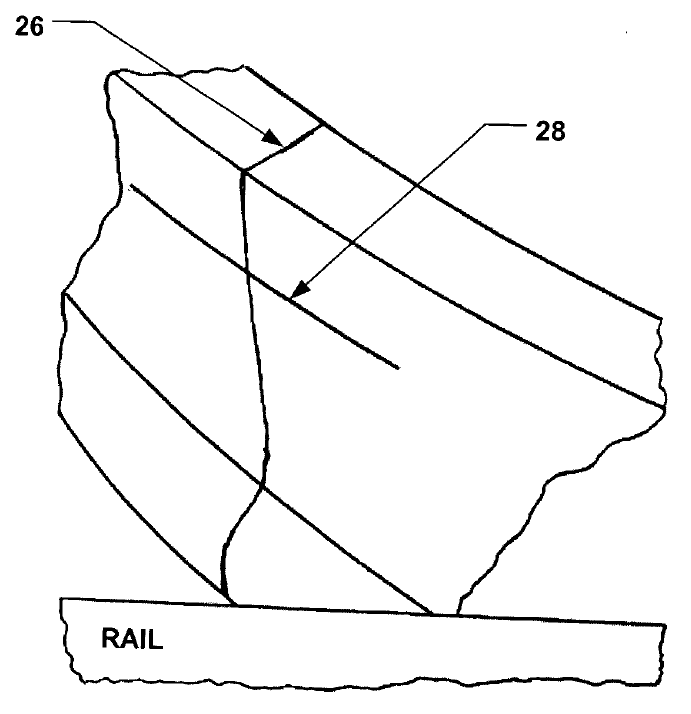
\includegraphics[width=0.6\textwidth]{./images/wpms/lasers1.png}
    \caption{System \#1, outer side collected sections}
    \label{fig:cmp-sys1}
  \end{figure}
Lasers lines are extracted from the (simultaneous) acquired images, after a preprocessing. This data elaboration consists of image resizing, laser spots detection, image equalization using threshold filters and rejection of noisy points. In particular, the detection of the laser spots is performed using edge-detection algorithms instead of subpixel filters; in this case the subpixel precision is guaranteed by the image resizing. Note that line 28 generally is not perpendicular to the axis of the wheel, because of the inclination of the same with respect to the rail. This situation introduces an error when we compute the diameter. Thus, the profile has to be projected in a plane perpendicular to the axis of the wheel, before compute the Equation \ref{eq:cylinder}. This correction is called \textit{radial compensation}. \\
The presentations of the commercial products of this corporation offer a precision greater of $96\%$ for each measure of interest (diameter, flange width and height, \ldots).

%%%
% If it is the case to do that, I've some other notes about BeenaVision
%%%


%%%%%%%%%%%%%%%%%%%%%%%%%%%
\subsubsection{System \#2} % Danobat
Differently from the previous system, this one proposes a method that can be used with many different structured light projectors, even if all proposed solutions are focused on laser stripes. This proposal basically uses at least two laser-camera pair in order to reconstruct the entire profile of the wheel, and solve the occlusion problem. \\
Once the laser spots are detected from the two different acquisitions, they are converted in a common 3D reference system, where $X$ is the longitudinal direction, $Y$ is the transverse direction and $Z$ the vertical direction. Converted data are then corrected, by aligning the profile with the ideal reference system: this corrects distortions due to the wheel inclination with respect to its axis (angle $\alpha$ and $\beta$, as shown in Figure \ref{fig:cmp-sys2}).
  \begin{figure}[t!]
    \centering
    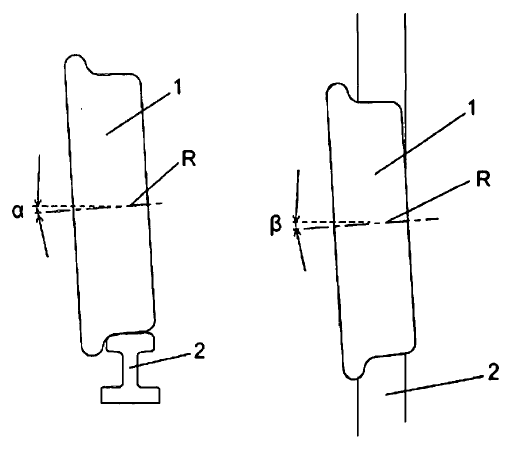
\includegraphics[width=0.7\textwidth]{./images/wpms/wheel-rotation.png}
    \caption{System \#2, wheel rotations with respect to ideal axis. $R$ is the ideal rotation axis, $1$ is the wheel and $2$ the rail.}
    \label{fig:cmp-sys2}
  \end{figure}
This is performed by correcting the rotation of the tensors parallel to the inner and outer side, with respect to the ideal ones. Furthermore this correction allows to analyse the profile in a well known position, regardless of how the profile is acquired by the camera (remember that the train is running on the sensor). At this point, for each detected laser spot, from the flange to the wheel contact surface, a radius is computed. Radius is understood as the distance between a point of light reflected on the section of the wheel and a transverse height $Y$ of the axis $R$ of the wheel, and it is computed using the equation:
  \begin{equation*}
    Radius = \sqrt{x^2 + z^2}
  \end{equation*}
where $x$ and $z$ are respectively the longitudinal and the transverse heights of each point of light of the laser line.
When all the parameters of interest are rough estimated, a Gauss-Newton algorithm is used in order to minimize the error on the computed radii, and in this way to refine the angles $\left( \alpha, \beta \right)$ and the position and orientation of each profile. At the end, the measures of interests are computed. The presentations of the commercial products of this corporation offer a precision around of $0.2 \, mm$ for measures concerning profile of the wheel (flange height and thickness, qR factor, \ldots) and a precision around of $1 \, mm$ for the diameter.
 
 
%%%%%%%%%%%%%%%%%%%%%%%%%%%
\subsubsection{System \#3} % IEM
Like the system \#2, also this approach is thought to be used both with laser beams and with structured light. Even the order with which the operations are performed is about the same:
  \begin{itemize}
    \item detection of the laser stripe;
    \item data conversion into the 3D $\left(XYZ\right)$ reference system and alignment to the ideal orientation;
    \item interpolation of the raw data using standard shape fitting algorithms;
    \item evaluation of the measures of interests.
  \end{itemize}
What distinguishes this system from others, is the approach used to detect the laser spot and to reconstruct the profile of the wheel. In fact, it uses standard geometric fitting algorithms to find each part that dial the profile, as flange, rim, wheel inner and outer sides, \ldots Once the entire profile is built from each acquired image (generally, one for each laser-camera pair used), the diameter of the wheel is determined using a standard circle fitting algorithm\footnote{Not specified in the patent} that allows to approximate the rolling circle. \\

Unfortunately, in the website of the manufacturer we have found only commercial description about the products, but no information about their precision, or accuracy. However, these informations could be meaningless. This corporation is the owner of many patents regarding laser-triangulation systems, each one of them proposes a different approach to the problem. For example, some of them are based on expert system or on neural network. Furthermore, different sensors are suggested, such as electromagnetic or acoustic devices. \\
All the patents analysed described a complete system, but avoid to study in details the algorithms used to process collected data, thus we can only speculate on how proposed systems really work.

%%%%%%%%%%%%%%%%%%%%%%%%%%%
\subsubsection{System \#4} % Mermec
Like the previous systems, also this last one is based on, at least, a couple of a laser-camera pair, that allow to reconstruct the entire profile of the wheel, similarly as shown in Figure \ref{fig:cmp-sys4}.
The laser beams are collected by the three cameras, and the spots are located using sup-pixel approximation algorithms, that increase the accuracy of the laser estimation, starting from the acquired images. Thus, the entire profile is rebuilt merging the inner and outer laser lines, and aligned to the ideal orientation. At this point, some keypoints are determined in order to evaluate the measures of interest. \\

One of the most meaningful points, is the rolling point: in fact it allows to estimate the diameter of the wheel. As in the previous case, this operation requires at least three points, taken from at least three synchronous acquisitions. Also in this case, a radial compensation is needed, in order to reduce the measurement error; if the system provides many triangulation groups, it is possible to estimate different diameters, and then average along this values. Note that, in this way it is possible to approximate the wheel circle, but it is not possible to consider wheel ovalization.
% Concerning the estimation of the diameter, given at least three different rolling points, belonging to the rebuilt profiles and taken in different positions, the Erone's formula is used:
%  \begin{equation*}
%    D = \frac{2\cdot a\cdot b\cdot c}{\sqrt{(a+b+c)(-a+b+c)(a-b+c)(a+b-c)}}
%  \end{equation*}
%where $a$, $b$ and $c$ are the sides of the triangle with vertexes the three point above. In this way it is possible to approximate the wheel circle, but it is not possible to consider wheel ovalizations.
  \begin{figure}[t!]
    \centering
    \begin{minipage}[c]{.49\textwidth}
      \centering
      %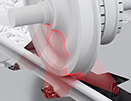
\includegraphics[width=\textwidth]{./images/wpms/mm-wpms.jpg}
      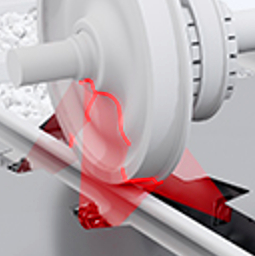
\includegraphics[width=0.8\textwidth]{./images/wpms/test2_cut.jpg}
    \end{minipage}%
    \hfill
    \begin{minipage}[c]{.49\textwidth}
      \centering
      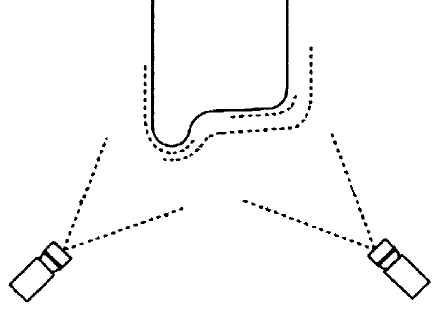
\includegraphics[width=\textwidth]{./images/wpms/laser_pts.png}
    \end{minipage}
    
    \caption{System \#4, example of system configuration.}
    \label{fig:cmp-sys4}
  \end{figure}

%%%%%%%%%%%%%%%%%%%%%%%%%%%
\subsubsection{System \#5} % \cite{wpms-giuseppe}
This last system proposes an alternative process to extract the laser stripe. Instead of improving the accuracy of the peak detection working on sub-pixel approximation, it uses an edge detector presented in \cite{chen2013efficient} and \cite{659930}. In this way, it is possible to detect the maximum of the second derivative of the grey level perpendicular to the laser stripe. Thus, it is possible to improve the peak detection even when the beam is not perpendicular to the pixel direction in the sensor, specially when the laser line bends (e.g. in the flange side). The system boast of reaching the precision of $0.1$ pieces of pixels, regardless of the variations in the width or light intensity (i.e. grey values) of the beam. Furthermore, the approach is more robust with respect to noise.

In order to correctly determine the diameter of the wheel, the system needs to rotate the profile, so that the rim plane segment can be parallel to the y-axis of the 2D coordinate frame on the laser plane. Hence, three rim plane segments can be determined, and using the 3D coordinates in the world reference system, it is possible to obtain the equation of the wheel rim plane by fitting all of the rim plane segments:
  \begin{equation}
    \pi_rim : a_rx + b_ry + c_rz + d_r = 0
    \label{eq:sys5-plane}
  \end{equation}
At the end, the diameter can be determined by projecting the flange vertexes and at least two contact points on the plane described in the Equation \ref{eq:sys5-plane}. Each of the point $p$ is projected in the rim plane accordingly with:
  \begin{equation*}
    p' = p + t\cdot\frac{N^T}{||N||}
  \end{equation*}
where $N = \begin{bmatrix} a_r, b_r, c_r \end{bmatrix}$, and $t$ is the distance from $p$ to the wheel rim plane. Thus, a maximum likelihood criterion is used against the noise, so as the approximation of the center of the wheel is improved, and a non-linear optimization method (e.g. Levenberg–Marquardt) can be performed to solve the problem. \\
The Levenberg–Marquardt algorithm (\acs{LMA} from the names of its inventors) is used to solve generic curve-fitting problems, and it always finds a local minima at least. This algorithm is slower that the Gauss-Newton one, but it is more precise. It is based on a least-squares method: given a set of $m$ empirical datum pairs $\left( x_i, y-i \right)$ of independent and dependent variables, find the parameters $\beta$ of the model curve $f(x,\beta)$ so that the sum of the squares of the deviations is minimized. \\

%%%%%%%%%%%%%%%%%%%%%%%%%%%
% Conclusion to the chapter
~\\

As we can see, the proposed systems are less than the number of the corporations analysed. As just mentioned before, many companies prefer to protect their products with corporation secrets instead using patents. Furthermore, many of the patents found are related to different systems or approaches (for example regarding static systems). These choices prevented us to comment all the products on the market. However, the systems discussed above, and summarised in Table \ref{tab:wpms:summaries}, are a good sample of the possible solutions for measuring the world using laser triangulation-based systems.
  % \caption{Summery of the systems above.}
% \label{tab:wpms:summaries}

\begin{table}[t!]
\footnotesize
\centering
\begin{tabular}{|l|p{4cm}|p{4cm}|l|}

\hline
\multicolumn{1}{|c|}{\textbf{\#}} & \multicolumn{1}{c|}{\textbf{Preprocessing}} & \multicolumn{1}{c|}{\textbf{Diameter}} & \multicolumn{1}{c|}{\textbf{Precision}} \\

\hline
\textit{1}  & * image resizing;                                                  & Profile radial                                                               & Higher than $96\%$  \\
            & * laser spots detection;                                           & compensation and                                                             &                     \\
            & * image equalization;                                              & approximation of the                                                         &                     \\
            & * rejection of noisy points.                                       & wheel to a cylinder                                                          &                     \\
			&                                                                    & instead of a cone.                                                           &                     \\
			&                                                                    &                                                                              &                     \\
			
\hline
\textit{2}  & * profiles extraction and                                          & Estimation of the center                                                     & $0.2 \, mm$ for measures \\
            & conversion in a common reference system;                           & of the wheel and computation of the radius for each                          & $1.0 \, mm$ for radius   \\
            & * profiles radial correction;                                      & rolling point. Application of a Gauss-Newton                                 &                          \\
            & * profiles merge.                                                  & algorithm to reduce the approximation error.                                 &                          \\
            &                                                                    &                                                                              &                          \\

\hline
\textit{3}  & * detection of the laser                                           & Standard circle fitting                                                      & $0.1 \, mm$ for measures \\
            & stripe;                                                            & algorithm                                                                    & $1.0 \, mm$ for radius   \\
            & * data conversion into the 3D reference system;                    &                                                                              &                          \\
            & * alignment to the ideal orientation;                              &                                                                              &                          \\
            & * data interpolation using shape fitting algorithms.               &                                                                              &                          \\
            &                                                                    &                                                                              &                          \\

\hline
\textit{4}  & * frame filtering;                                                 & Evaluation through                                                           & Not found           \\
            & * profile extraction;                                              & rolling points                                                               &                     \\
            & * conversion into 3D reference system;                             &                                                                              &                     \\
            & * profiles merge;                                                  &                                                                              &                     \\
            & * performing of radial compensation to the profile.                &                                                                              &                     \\
            &                                                                    &                                                                              &                     \\

\hline
\textit{5}  & * Profile extraction using edge detector algorithms.               & * Alignment of the profile to the reference system;                      & Not found               \\
            &                                                                    & * fitting of the wheel rim plane;                                        &                         \\
            &                                                                    & * projection of the flange on the plane;                                 &                         \\
            &                                                                    & * use of a maximum likelihood algorithm to reduce the error.             &                         \\
\hline
\end{tabular}

\caption{Summery of the systems above.}
\label{tab:wpms:summaries}
\end{table}
%  \begin{table}
%    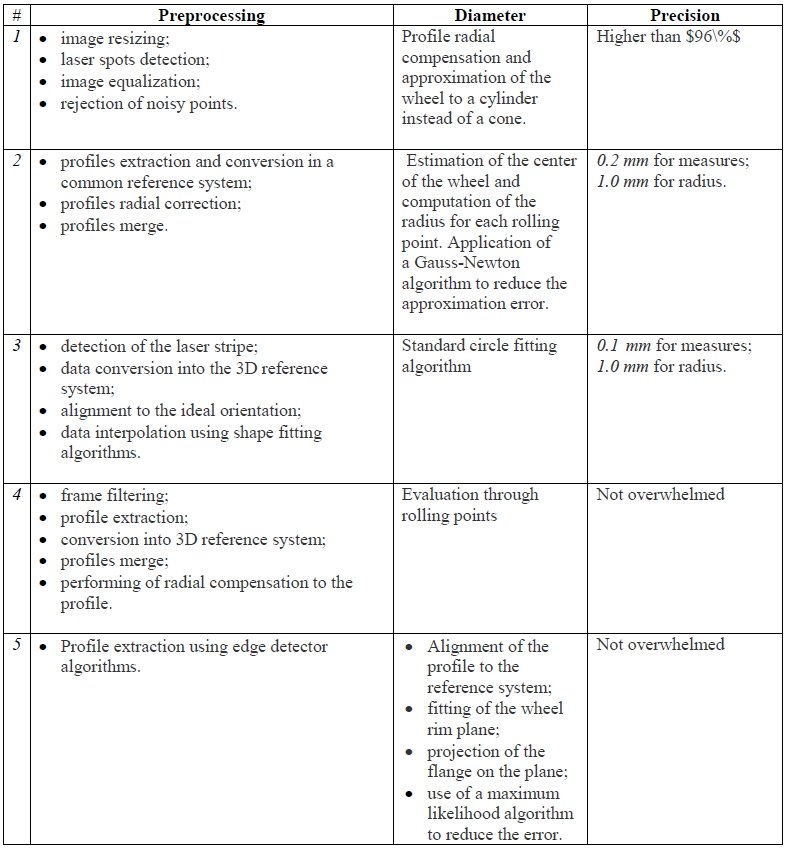
\includegraphics[width=\textwidth]{./images/wpms/tab.PNG}
%    \caption{Summery of the systems above.}
%    \label{tab:wpms:summaries}
%  \end{table}